% Options for packages loaded elsewhere
\PassOptionsToPackage{unicode}{hyperref}
\PassOptionsToPackage{hyphens}{url}
\PassOptionsToPackage{dvipsnames,svgnames,x11names}{xcolor}
%
\documentclass[
  12pt]{article}

\usepackage{amsmath,amssymb}
\usepackage{iftex}
\ifPDFTeX
  \usepackage[T1]{fontenc}
  \usepackage[utf8]{inputenc}
  \usepackage{textcomp} % provide euro and other symbols
\else % if luatex or xetex
  \usepackage{unicode-math}
  \defaultfontfeatures{Scale=MatchLowercase}
  \defaultfontfeatures[\rmfamily]{Ligatures=TeX,Scale=1}
\fi
\usepackage{lmodern}
\ifPDFTeX\else  
    % xetex/luatex font selection
\fi
% Use upquote if available, for straight quotes in verbatim environments
\IfFileExists{upquote.sty}{\usepackage{upquote}}{}
\IfFileExists{microtype.sty}{% use microtype if available
  \usepackage[]{microtype}
  \UseMicrotypeSet[protrusion]{basicmath} % disable protrusion for tt fonts
}{}
\makeatletter
\@ifundefined{KOMAClassName}{% if non-KOMA class
  \IfFileExists{parskip.sty}{%
    \usepackage{parskip}
  }{% else
    \setlength{\parindent}{0pt}
    \setlength{\parskip}{6pt plus 2pt minus 1pt}}
}{% if KOMA class
  \KOMAoptions{parskip=half}}
\makeatother
\usepackage{xcolor}
\setlength{\emergencystretch}{3em} % prevent overfull lines
\setcounter{secnumdepth}{5}
% Make \paragraph and \subparagraph free-standing
\ifx\paragraph\undefined\else
  \let\oldparagraph\paragraph
  \renewcommand{\paragraph}[1]{\oldparagraph{#1}\mbox{}}
\fi
\ifx\subparagraph\undefined\else
  \let\oldsubparagraph\subparagraph
  \renewcommand{\subparagraph}[1]{\oldsubparagraph{#1}\mbox{}}
\fi


\providecommand{\tightlist}{%
  \setlength{\itemsep}{0pt}\setlength{\parskip}{0pt}}\usepackage{longtable,booktabs,array}
\usepackage{calc} % for calculating minipage widths
% Correct order of tables after \paragraph or \subparagraph
\usepackage{etoolbox}
\makeatletter
\patchcmd\longtable{\par}{\if@noskipsec\mbox{}\fi\par}{}{}
\makeatother
% Allow footnotes in longtable head/foot
\IfFileExists{footnotehyper.sty}{\usepackage{footnotehyper}}{\usepackage{footnote}}
\makesavenoteenv{longtable}
\usepackage{graphicx}
\makeatletter
\def\maxwidth{\ifdim\Gin@nat@width>\linewidth\linewidth\else\Gin@nat@width\fi}
\def\maxheight{\ifdim\Gin@nat@height>\textheight\textheight\else\Gin@nat@height\fi}
\makeatother
% Scale images if necessary, so that they will not overflow the page
% margins by default, and it is still possible to overwrite the defaults
% using explicit options in \includegraphics[width, height, ...]{}
\setkeys{Gin}{width=\maxwidth,height=\maxheight,keepaspectratio}
% Set default figure placement to htbp
\makeatletter
\def\fps@figure{htbp}
\makeatother

\addtolength{\oddsidemargin}{-.5in}%
\addtolength{\evensidemargin}{-1in}%
\addtolength{\textwidth}{1in}%
\addtolength{\textheight}{1.7in}%
\addtolength{\topmargin}{-1in}%
\makeatletter
\makeatother
\makeatletter
\makeatother
\makeatletter
\@ifpackageloaded{caption}{}{\usepackage{caption}}
\AtBeginDocument{%
\ifdefined\contentsname
  \renewcommand*\contentsname{Table of contents}
\else
  \newcommand\contentsname{Table of contents}
\fi
\ifdefined\listfigurename
  \renewcommand*\listfigurename{List of Figures}
\else
  \newcommand\listfigurename{List of Figures}
\fi
\ifdefined\listtablename
  \renewcommand*\listtablename{List of Tables}
\else
  \newcommand\listtablename{List of Tables}
\fi
\ifdefined\figurename
  \renewcommand*\figurename{Figure}
\else
  \newcommand\figurename{Figure}
\fi
\ifdefined\tablename
  \renewcommand*\tablename{Table}
\else
  \newcommand\tablename{Table}
\fi
}
\@ifpackageloaded{float}{}{\usepackage{float}}
\floatstyle{ruled}
\@ifundefined{c@chapter}{\newfloat{codelisting}{h}{lop}}{\newfloat{codelisting}{h}{lop}[chapter]}
\floatname{codelisting}{Listing}
\newcommand*\listoflistings{\listof{codelisting}{List of Listings}}
\makeatother
\makeatletter
\@ifpackageloaded{caption}{}{\usepackage{caption}}
\@ifpackageloaded{subcaption}{}{\usepackage{subcaption}}
\makeatother
\makeatletter
\@ifpackageloaded{tcolorbox}{}{\usepackage[skins,breakable]{tcolorbox}}
\makeatother
\makeatletter
\@ifundefined{shadecolor}{\definecolor{shadecolor}{rgb}{.97, .97, .97}}
\makeatother
\makeatletter
\makeatother
\makeatletter
\makeatother
\ifLuaTeX
  \usepackage{selnolig}  % disable illegal ligatures
\fi
\usepackage[]{natbib}
\bibliographystyle{agsm}
\IfFileExists{bookmark.sty}{\usepackage{bookmark}}{\usepackage{hyperref}}
\IfFileExists{xurl.sty}{\usepackage{xurl}}{} % add URL line breaks if available
\urlstyle{same} % disable monospaced font for URLs
\hypersetup{
  pdftitle={Is US Debt Brinkmanship a Debt Crisis Without Default?},
  pdfauthor={William Clinton Co},
  pdfkeywords={3 to 6 keywords, that do not appear in the title},
  colorlinks=true,
  linkcolor={blue},
  filecolor={Maroon},
  citecolor={Blue},
  urlcolor={Blue},
  pdfcreator={LaTeX via pandoc}}


\begin{document}


\def\spacingset#1{\renewcommand{\baselinestretch}%
{#1}\small\normalsize} \spacingset{1}


%%%%%%%%%%%%%%%%%%%%%%%%%%%%%%%%%%%%%%%%%%%%%%%%%%%%%%%%%%%%%%%%%%%%%%%%%%%%%%

\date{July 2, 2023}
\title{\bf Is US Debt Brinkmanship a Debt Crisis Without Default?}
\author{
William Clinton Co\thanks{We would like to express my gratitude to
Jonathan Graves for helpful feedback ,guidance and the opportunity to
participate.}\\
Department of Economics, The University of British Columbia\\
}
\maketitle

\bigskip
\bigskip
\begin{abstract}
Under the backdrop of increasing public debt, ``debt crisis without
default'' and safe asset shortages, we investigate how US debt
brinkmanship plays a role into mentioned topics.
\end{abstract}

\noindent%
{\it Keywords:} 3 to 6 keywords, that do not appear in the title
\vfill

\newpage
\spacingset{1.9} % DON'T change the spacing!
\ifdefined\Shaded\renewenvironment{Shaded}{\begin{tcolorbox}[boxrule=0pt, frame hidden, borderline west={3pt}{0pt}{shadecolor}, sharp corners, interior hidden, breakable, enhanced]}{\end{tcolorbox}}\fi

\hypertarget{sec-l}{%
\section{Literature}\label{sec-l}}

\hypertarget{increasing-public-debt}{%
\subsection{Increasing Public Debt}\label{increasing-public-debt}}

Constantly increasing public debt has been a recent developmet
throughout recent history \citep{mitchener2023}. This raises the
question of how will governments deal with rising debt burdens going
forward. As debt increases, cost of borrowing increases. Will
governments internalize the increase of cost of borrowing?

\hypertarget{debt-crisis-without-default}{%
\subsection{Debt Crisis Without
Default}\label{debt-crisis-without-default}}

It has also been noted we have debt crisis without default has become
more common, wherein there was a near missed payment but never a default
has a negative effect on output, as exemplified in Greece Portugal and
Spain during 2010-2012 \citep{mitchener2023} . Going a step further some
have propose to change the definition of debt crises to yield spreads of
1000 basis points, also known as spread spikes
\citep{broner2013, aguiar, krishnamurthy}.

What makes this even more poignant is that the output decline happens in
anticipation of a default rather than the default itself
\citep{yeyati2011}.

What makes this an important topic to study is the body of evidence
proving a decline in output associated with the high yields that
accompanies a debt crisis. There are varying reasons for this such as
the relationship between external financing and importers
\citep{mendoza2012}, the decrease in external domestic firm
borrowing\citep{corsetti2012, das2010, gourinchas2016} or the tightening
of credit against loses on bank balance
sheets\citep{arellano, ferrando2017}.

There has also been work on how credit rating agencies downgrading
reduces leverage and investments \citep{almeida2017}. Similar
conclusions were drawn using CDS risk premium instead of bond yield
spreads \citep{brutti2015, bahaj2020}. Similarly, we explore this in the
context of debt brinkmanship.

Interestingly, the current literature has yet to consider if US debt
ceiling brinkmanship falls under this category.

\hypertarget{safe-asset-shortage}{%
\subsection{Safe Asset Shortage}\label{safe-asset-shortage}}

Another pertinent question is the many creditors willing to lend to
highly indebted sovereigns. Currently we are in a safe asset shortage,
such that we are coming closer to the effective lower bound, wherein
central banks could not decrease interest rates any further as needed.
This shortage is a key source of fragility in the economy, dubbed the
``safety trap'' \citep{caballero2017} . Similarly, the current
literature has yet to consider if US debt ceiling brinkmanship
contributes to this phenomenon.

\hypertarget{introduction}{%
\section{Introduction}\label{introduction}}

The US treasury yield occupies the status as the biggest and most liquid
market, wherein its yield is a significant determinant of yields
globally. This phenomenon would be described as the ``global factor''
becoming increasingly more important determinant of yields ,against
specific ``country'' factors \citep{mauro2002}. Thus, studying the
properties of US' yields would be important.
\citep{rozada2006, gonzález-rozada2008, longstaff2011}. We shall study
US' yields in the context of debt ceiling brinkmanship. Furthermore,
current literature on debt focuses on events like Greece or Argentina,
less work has been done with consideration to US debt ceiling.

\hypertarget{public-debt-and-debt-brinkmanship}{%
\subsection{Public Debt and Debt
Brinkmanship}\label{public-debt-and-debt-brinkmanship}}

Previous literature etablishes the recent development of increasing high
public debt{[} \citet{mitchener2023} {]}. While others note that debt
brinkmanship has become more and more worse \citep{berman} , evident by
the increasing trend of passing debt limit suspension vs raises.
Insiders and analyst mention how normalized brinkmanship has become
\citep{bivens} . We investigate the link between the two.

We plot US debt limit increases along with world global change in
debt/GDP ratios. We also plot the frequency of debt raises/suspensions
to identify trends. We will also take note of rating agency negative
outlooks from the top 3 rating agencies. Taking inspiration from

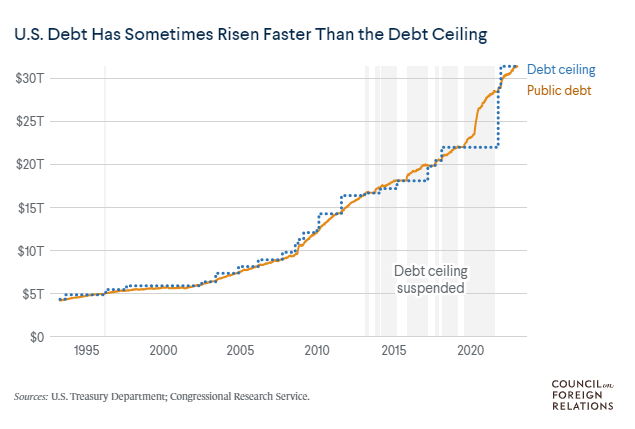
\includegraphics[width=4.8125in,height=\textheight]{style-guide/Debt plot.png}

\hypertarget{how-will-governments-react-to-the-increasing-cost-of-borrowing}{%
\subsection{How will governments react to the increasing cost of
borrowing?}\label{how-will-governments-react-to-the-increasing-cost-of-borrowing}}

We construct a data set of X-dates, dates where the US government will
supposedly run out of money. This is done by analyzing the maximum ex
ante yield spread and CDS prices. We then analyze changes in CDS prices
and yields, using data from Bloomberg. We use official whitehouse data
to get dates of debt limit increase. We build on prior work which uses
the 1000 basis points as a benchmark. We isolate brinkmanship with a
1000 basis point increase against those without. An example would be

\begin{longtable}[]{@{}
  >{\raggedright\arraybackslash}p{(\columnwidth - 10\tabcolsep) * \real{0.1351}}
  >{\raggedright\arraybackslash}p{(\columnwidth - 10\tabcolsep) * \real{0.1757}}
  >{\raggedright\arraybackslash}p{(\columnwidth - 10\tabcolsep) * \real{0.2027}}
  >{\raggedright\arraybackslash}p{(\columnwidth - 10\tabcolsep) * \real{0.1351}}
  >{\raggedright\arraybackslash}p{(\columnwidth - 10\tabcolsep) * \real{0.1892}}
  >{\raggedright\arraybackslash}p{(\columnwidth - 10\tabcolsep) * \real{0.1622}}@{}}
\toprule\noalign{}
\begin{minipage}[b]{\linewidth}\raggedright
X-date
\end{minipage} & \begin{minipage}[b]{\linewidth}\raggedright
Date of Increase
\end{minipage} & \begin{minipage}[b]{\linewidth}\raggedright
Negotiation length=(X-date)-Date of Increase
\end{minipage} & \begin{minipage}[b]{\linewidth}\raggedright
CDS
\end{minipage} & \begin{minipage}[b]{\linewidth}\raggedright
CDS1000(1000 basis points or more)
\end{minipage} & \begin{minipage}[b]{\linewidth}\raggedright
Yields
\end{minipage} \\
\midrule\noalign{}
\endhead
\bottomrule\noalign{}
\endlastfoot
\(x_1\) & \(d_1\) & \(n_{1,yes}=x_1-d_1\) & \(c_1\) & yes & \(y_1\) \\
\(x_2\) & \(d_2\) & \(n_{1,no}=x_2-d_2\) & \(c_2\) & no & \(y_2\) \\
\ldots. & \ldots.. & \ldots. & \ldots.. & \ldots.. & \ldots{} \\
\end{longtable}

We investigate if debt ceiling negotiations settle faster given a sharp
increase in cost. We compute \(\bar{n_{y}}\) , average negotiation
length with a spread spike and compare this to \(\bar{n_{n}}\),
negotiation length with no spike.

We also run regression
\(NegoLength=\beta_1\Delta CDS+\beta_2\Delta Yields+\beta_3D_{neg-outlook}\),
such that we investigate weather debt ceiling negotiations will settle
earlier given a bigger increased in cost of capital. We split cost of
capital into three components CDS prices, yields and rating agency
downgrades.

We investigate trends overtime by \textbf{plotting} negation length on
the y axis against date of increase on the x axis.

We study how brinkmanship affects country yield spreads. we take
inspiration from the data set by \citep{meyer2022} as it relates data on
debt ceiling brinkmanship \citep{reinhart2008}.

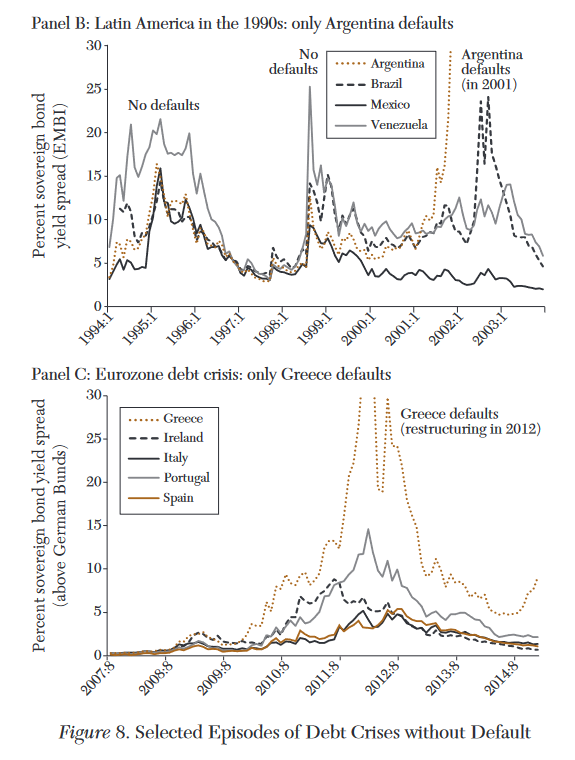
\includegraphics[width=3.94792in,height=\textheight]{style-guide/overtime_brink_2.png}

\hypertarget{contributor-to-safe-asset-shortage}{%
\subsection{Contributor to safe asset
shortage?}\label{contributor-to-safe-asset-shortage}}

Ever since the 2008 financial crisis risk premiums have not returned to
prior levels\citep{caballero2017}.We investigate if debt brinkmanship
contributes to this phenomenon as well. If so then there would be an
argument to abolish the system on a global welfare standpoint. We take
inspiration from

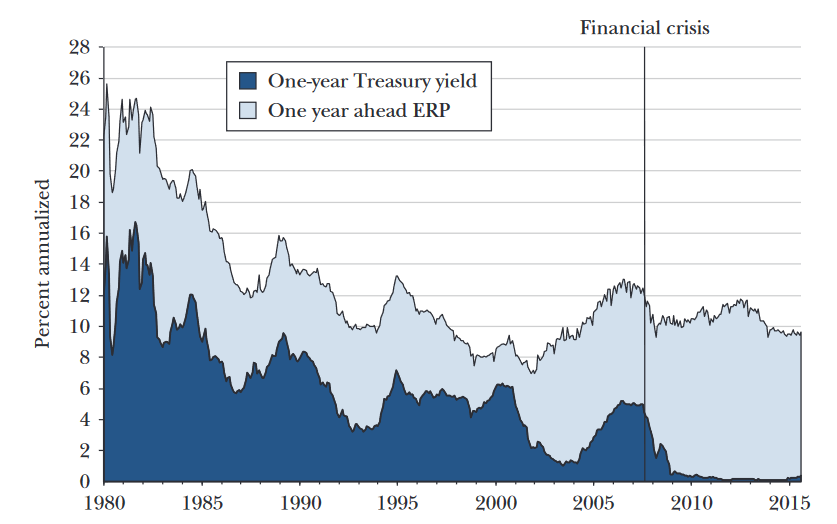
\includegraphics[width=6.10417in,height=\textheight]{style-guide/1_year_ERP.png}

We construct a similar graph as above taking debt ceiling dates.

Using time t, as the time of debt increase. We graph a line representing
the average change in 1 year expected risk premium. Another line
represents the average change in 1 year treasury yields. We construct
the graph below with mentioned variables \citep{duarte2015}.

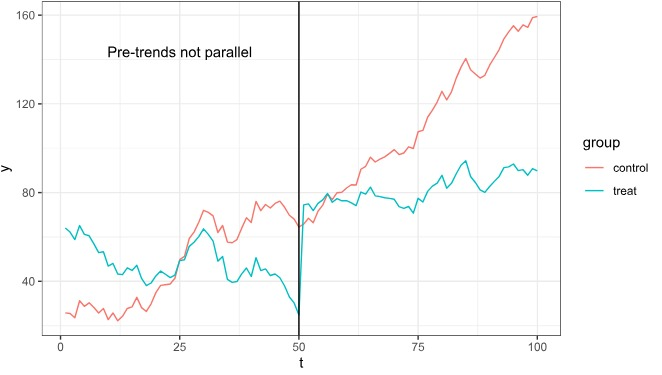
\includegraphics[width=5.21875in,height=\textheight]{style-guide/1_year_ERP_parallel_trends.jpeg}

\hypertarget{debt-crisis-without-default-1}{%
\subsection{Debt Crisis without
Default?}\label{debt-crisis-without-default-1}}

We then investigate if debt ceiling brinkmanship can be characterized as
a debt crisis without default, as defined by prior literature. We graph

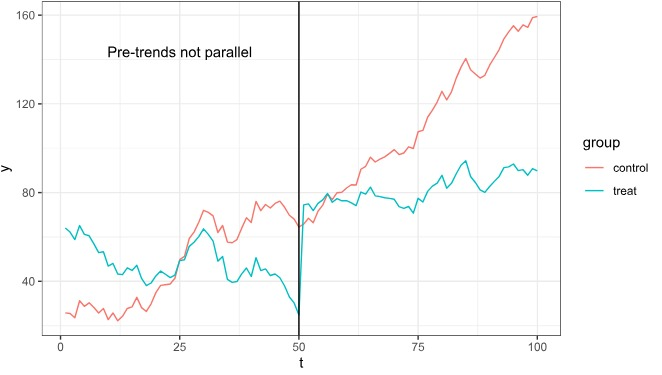
\includegraphics[width=4.875in,height=\textheight]{style-guide/1_year_ERP_parallel_trends.jpeg}

the y axis would represent GDP. We then make 3 lines corresponding to
the following attributes advanced countries, developing countries and
China. We will use IMF definition and ifs dataset to accomplish this. We
investigate if the output decline show by \citep{yeyati2011} is present.
We also propose a similar graph using imports on the y axis in line with
\citep{mendoza2012}. We investigate debt to market cap levels fo firms
\citep{corsetti2012, das2010, gourinchas2016}s. We investigate
investments \citep{almeida2017}

We consider China for the follwing reasons. China's rise to the world
stage has been marked with capital exports that significantly alter
global yields \citep{alfaro2014, gourinchas}. In fact, China's lending
portfolio surpasses that of the World Bank \citep{horn2021} . We use
horns data-set. to analyze this.

US debt brinkmanship has been getting more fierce.

\hypertarget{sec-dataset}{%
\section{Data set}\label{sec-dataset}}


\renewcommand\refname{References}
  \bibliography{bibliography.bib}


\end{document}
